\documentclass[12pt,a4paper]{article}
\usepackage[utf8]{inputenc}
\usepackage[left=2.5cm,right=2.5cm,top=3cm,bottom=2cm]{geometry}
\author{Pauline Speckmann}
\usepackage{graphicx}

\usepackage{fancyhdr}
\pagestyle{fancy}
\fancyhf{}
\fancyhead[l]{Digitalisierung Vorlesung 1 $-$ Zusammenfassung von Pauline Speckmann}
\fancyhead[r]{\thepage}

\begin{document}
\section{Informationssysteme als Gestaltungsgegenstand der Digitalisierung}


\vspace*{1cm}
\subsection{Digitalisierung} %%%%%%%%%%%%%%%%%%%%%%%%%%%%%%%%%%%%%%%%%%%%%%%%%%%%%%%%%%%%%%%%%%%%%%%%%%%%%%%%%%%%%%%%%%%%%%%%%%%%

\begin{itemize}
    \item \textbf{Begrifflichkeiten}:
       \begin{itemize}
          \item \textbf{Digitization}: Digitalisierung von Daten \\
		          Die Umwandlung von analogen in digitale Produkte und Dienstleistungen
		    \item \textbf{Digitalization}: Digitalisierung der Wertschöpfung \\
		          Die Veränderung von Geschäftsprozessen durch digitale Technologien
		    \item \textbf{Digitale Transformation}: \\
		          Die Neuorganisation von Geschäftsmodellen und Industrien durch digitale Technologien
       \end{itemize}
    
    \item \textbf{Der Einfluss der Digitalisierung auf die Organisation (Auswahl)}:
       \begin{itemize}
		    \item Abnehmende Distanz zwischen IT und Realität
		    \item Moorsches Gesetz
		    \item Kapselung von Funktionalitäten
		    \item KI-Entwicklung 
		\end{itemize}
\end{itemize}


\vspace*{0.8cm}
\subsection{Wirtschaftsinformatik} %%%%%%%%%%%%%%%%%%%%%%%%%%%%%%%%%%%%%%%%%%%%%%%%%%%%%%%%%%%%%%%%%%%%%%%%%%%%%%%%%%%%%%%%%%%%%%

\begin{itemize}
   \item \textbf{Was ist Ziel der Wirtschaftsinformatik?}\\
         Die Gestaltung von sozial akzeptablen, technisch stabilen und ökonomisch nachhaltigen Informationssystemen.
   
   \item \textbf{Paradigmen der Wirtschaftsinformatik:}
   \begin{itemize}
      \item \textbf{Realwissenschaft}: \\
            Einsatz von Informationssystemen in Wirtschaft, Verwaltung und dem privaten Lebensumfeld\\
            Schwerpunkt: Untersuchung von Einflüssen von IS im Unternehmen\\
            $\rightarrow$ Forschungsgegenstand sind reale Sachverhalte
      \item \textbf{Formalwissenschaft}: \\
            Entwicklung und Anwendung formaler Beschreibungsverfahren und Theorien 
            (bspw. zur Reduzierung der Komplexität (Modellierung))\\
            $\rightarrow$ Abstrakte Inhalte als Forschungsgegenstand
      \item \textbf{Ingenieurwissenschaft}: \\
            Gestaltung betrieblicher Informationssysteme\\
            $\rightarrow$ Technik und Entwicklung dieser
   \end{itemize}
\end{itemize}
 

\subsection{Informationssysteme} %%%%%%%%%%%%%%%%%%%%%%%%%%%%%%%%%%%%%%%%%%%%%%%%%%%%%%%%%%%%%%%%%%%%%%%%%%%%%%%%%%%%%%%%%%%%%%%%

\begin{itemize}
   \item \textbf{Definition}:\\
         Bei Informationssystemen handelt es sich um soziotechnische (Mensch-Maschine) Systeme, die menschliche und maschinelle Komponenten (Teilsysteme) umfassen, insbesondere einer Aufgabenerfüllungdienen und zum Ziel der optimalen Bereitstellung von Informationen, Koordination und Kommunikation nach wirtschaftlichen Kriterien eingesetzt werden.

   \item \textbf{Charakteristika}:
      \begin{itemize}
         \item besteht aus Menschen und/oder Maschinen
         \item erzeugt oder benutzt Informationen
         \item verbindet Akteure durch Kommunikationsbeziehungen miteinander
      \end{itemize}
         
   \item \textbf{Ziele der Informationssysteme}:
			\begin{itemize}
			    \item Planung, Steuerung und Kontrolle in der Organisation unterstützen
			    \item Geschäftsprozesse beschleunigen
			    \item Qualität und Service verbessern
			    \item Wettbewerbsvorteile generieren
			\end{itemize}
   
   \item \textbf{Zentrale Begriffe, Normen und Abgrenzungen}:
         \begin{center}
            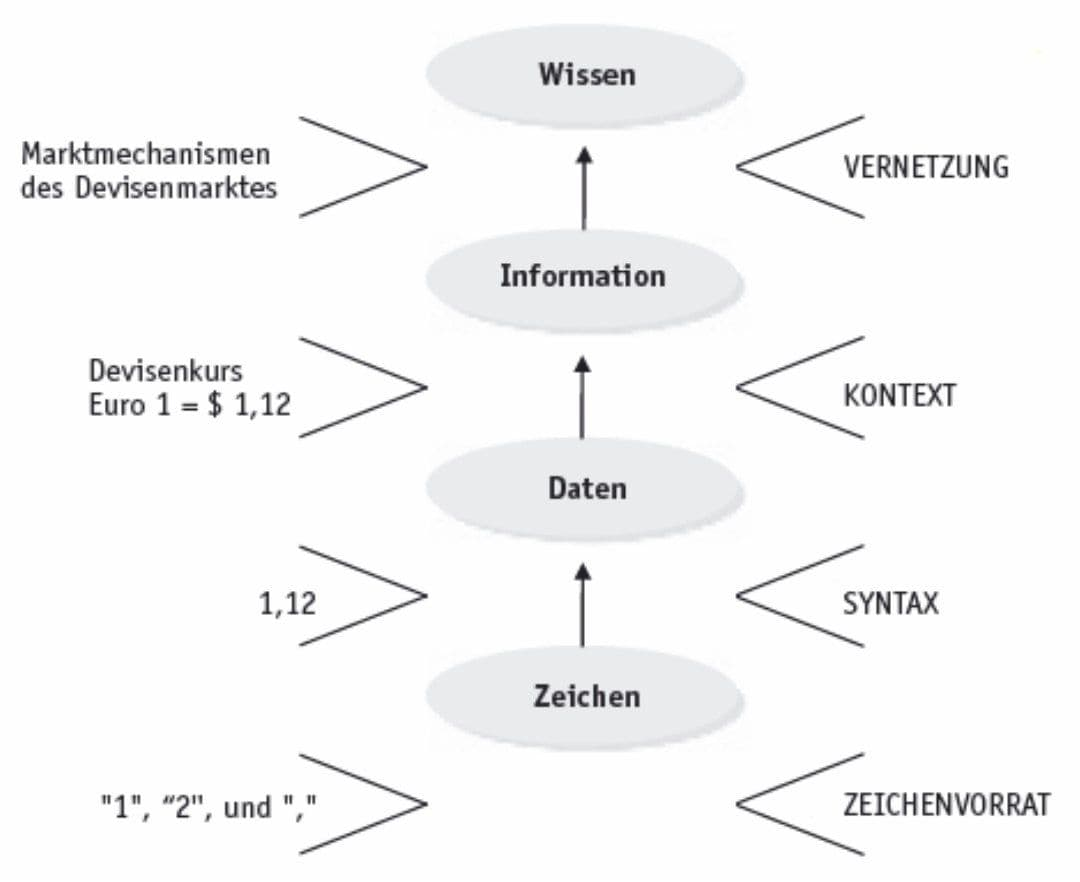
\includegraphics[scale=0.6]{ZentraleBegriffe-Normen-Abgrenzungen.jpg}
         \end{center}

\newpage %Manuelle Formatierung
   \item \textbf{Teilsysteme in Unternehmen}:
         \begin{center}
            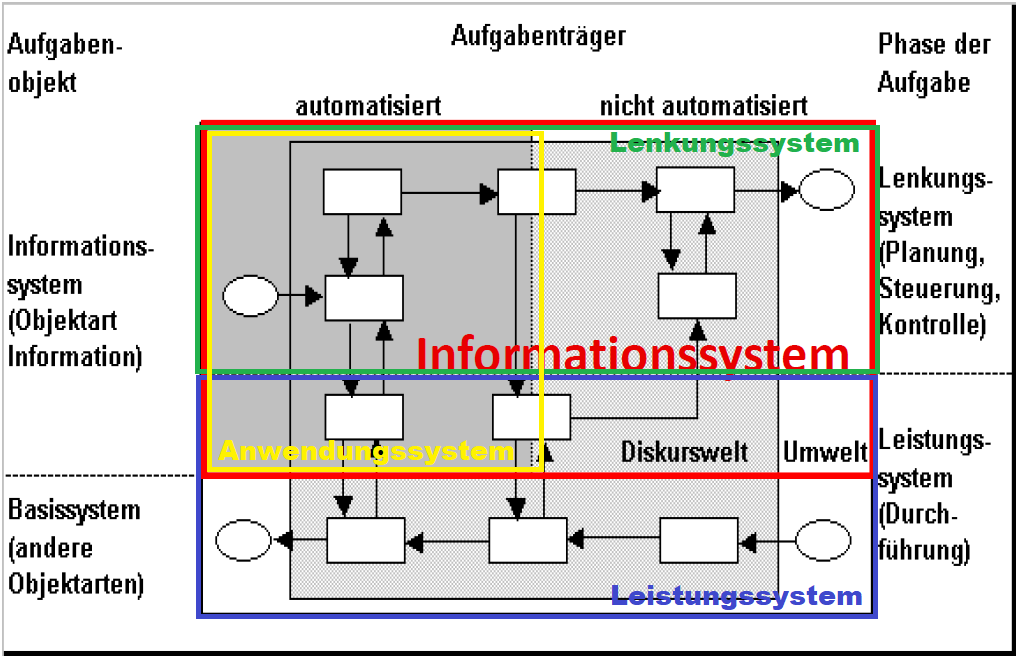
\includegraphics[scale=0.55]{Teilsysteme-in-Unternehmen.png}
         \end{center}
   
   \item \textbf{Ziele der Informationslogistik}:
         \begin{itemize}
            \item richtige Information (aktuell benötigt, verstanden, fehlerfrei)
            \item richtiger Zeitpunkt (Just in time (JIT))
            \item richtige Menge (so viel wie nötig, so wenig wie möglich)
            \item richtiger Ort (beim Empfänger verfügbar)
            \item erforderliche Qualität (ausreichend detailliert und wahr, unmittelbar verwendbar)
         \end{itemize}

   \item \textbf{Grundfragen bei der Gestaltung von Informationssystemen}:
      \begin{itemize}
         \item \textit{Wozu} (Auswertungszweck) wird die Information gebraucht?
         \item \textit{Wer} soll \textit{wen} über \textit{was} (Inhalt, Genauigkeit) informieren?
         \item \textit{Wann} (Termine) soll informiert werden?
         \item \textit{Wie} (Art, Form, Methode, Weg) soll informiert werden?
      \end{itemize}
\end{itemize}

\end{document}